%
% chapter.tex -- Graphenbeschreibung mit Matrizen
%
% (c) 2020 Prof Dr Andreas Müller, Hochschule Rapperswil
%
\chapter{Graphen
\label{buch:chapter:graphen}}
\lhead{Graphen}
\rhead{}
Ein Graph ist eine Menge von Knoten, die untereinander mit Kanten
verbunden sind.
Graphen können zum Beispiel verwendet werden um Netzwerke zu beschreiben,
aber auch viele andere Datenstrukturen.
\index{Graph}%
Die Knoten können einzelne Objekte beschreiben, die Kanten beschreiben
dann Beziehungen zwischen diesen Objekten.
Graphen haben zwar nur eine eindimensionale Geometrie, sie können aber auch als
erste Approximation dreidimensionaler Objekte dienen.

Die Bedeutung des Graphenkozeptes wird unterstrichen von der Vielzahl
von Fragestellungen, die über Graphen gestellt, und der
zugehöriten Lösungsalgorithmen, die zu ihrer Beantwortung gefunden
worden sind.
Die Komplexitätstheorie hat sogar gezeigt, dass sich jedes diskrete
Problem in ein Graphenproblem umformulieren lässt.
\index{Komplexitätstheorie}%

Das Problem, einen Stundenplan zu finden, der sicherstellt, dass
alle Studierenden jedes Fach besuchen können, für die sie sich
angemeldet haben, lässt sich zum Beispiel wie folgt als ein
Graphenproblem formulieren.
Die Fächer betrachten wir als Knoten des Graphen.
Für jedes Paar von Fächern ziehen wir eine Kante des Graphen, wenn 
sich mindestens ein Studierender für beide Fächer angemeldet hat.
Die Kante drückt aus, dass die beiden Fächer nicht zur gleichen Zeit
geplant werden dürfen.
Das Problem, einen Stundenplan zu finden, besteht jetzt darin, für
jedes Fach ein Zeitintervall zu finden, während dem es durchgeführt
werden soll.
\index{Stundenplan}%
Natürlich steht nur eine beschränkte Anzahl Zeitintervalle zur Verfügung
und benachbarte Knoten dürfen nicht ins gleiche Zeitintervall geplant
werden.
Das zugehörige abstrakte Graphenproblem heisst das Färbeproblem: 
\index{Färbeproblem}%
ist es möglich, mit einer beschränkten Anzahl von Farben die Knoten
des Graphen so einzufärben, dass benachbarte Knoten niemals die gleiche
Farbe haben.

In diesem Kapitel soll zunächst gezeigt werden, wie man Graphen mit 
Hilfe von Matrizen beschreiben kann
(Abschnitt~\ref{buch:section:beschreibung-von-graphen-mit-matrizen}).
Das Ziel dabei ist natürlich, die Hilfsmittel der Matrixalgebra
zur Lösung von Graphenprobleme hinzuzuziehen.
Die spektrale Graphentheorie in
Abschnitt~\ref{buch:section:spektrale-graphentheorie} verwendet
die Eigenwerte und Eigenvektoren der zugehörigen Matrix, um Aussagen
über den Graphen zu machen.
\index{Graphentheorie!spektrale}%
In Abschnitt~\ref{buch:section:wavelets-auf-graphen} wird gezeigt,
wie spektralen Eigenschaften verwendet werden können, um eine
Art von Wavelets auf einem Graphen zu definieren.
Damit ensteht eine für gewisse Anwendungen besonders leistungsfähige
Basis zur Beschreibung von Funktionen auf dem Graphen.

%
% beschreibung.tex -- Beschreibung von Graphen mit Matrizen
%
% (c) 2020 Prof Dr Andreas Müller, Hochschule Rapperswil
%
\section{Beschreibung von Graphen mit Matrizen
\label{buch:section:beschreibung-von-graphen-mit-matrizen}}
\rhead{Beschreibung mit Matrizen}
Ein Graph ist eine Menge von Knoten, die untereinander mit Kanten
verbunden sind.
Graphen können zum Beispiel verwendet werden um Netzwerke zu beschreiben,
aber auch viele andere Datenstrukturen.
Die Knoten können einzelne Objekte beschreiben, die Kanten beschreiben
dann Beziehungen zwischen diesen Objekten.

\subsection{Definition von Graphen
\label{subsection:definition-von-graphen}}
In der Einleitung zu diesem Abschnitt wurde bereits eine informelle
Beschreibung des Konzeptes eines Graphen gegeben.
Um zu einer Beschreibung mit Hilfe von Matrizen zu kommen,
wird eine exakte Definition benötigt.
Dabei werden sich einige Feinheiten zeigen, die für Anwendungen wichtig
sind und sich in Unterschieden in der Definition der zugehörigen Matrix 
äussern.

\subsubsection{Ungerichtete Graphen}
Die Grundlage für alle Arten von Graphen ist eine Menge $V$ von {\em Knoten},
auch {\em Vertices} genannt.
\index{Knoten}%
\index{Vertex}%
Die Unterschiede zeigen sich in der Art und Weise, wie die Knoten
mit sogenannten Kanten
\index{Kante}%
verbunden werden.
Bei einen ungerichteten Graphen sind die beiden Endpunkte einer Kante
gleichwertig, es gibt keine bevorzugte Reihenfolge oder Richtung der
Kante.
Eine Kante wird daher vollständig spezifiziert, wenn wir die
Menge der Endpunkte kennen.
Dies führt auf die folgende Definition eines ungerichteten Graphen.

\begin{definition}
\label{buch:def:ungerichteter-graph}
\index{Graph!ungerichteter}%
\index{ungerichteter Graph}%
Ein {\em ungerichteter Graph} ist eine endliche Menge $V$ von {\em Knoten}
und eine Menge $E$ von zweielementigen Teilmengen 
\[
E \subset \{\, \{a,b\}\subset V\,|\, a\ne b\}.
\]
Die Elemente von $E$ heissen {\em Kanten} ({\em edges}).
\end{definition}

Man beachte, dass es keine Kante gibt, die einen Knoten $a\in V$
mit sich selbst verbindet, da die zugehörige Menge $\{a,a\}=\{a\}$
nicht aus zwei verschiedenen Elementen besteht, wie die
Definition~\ref{buch:def:ungerichteter-graph} dies verlangt.

Ein elektrisches Netzwerk von ohmschen Widerständen kann mit Hilfe
eines ungerichteten Graphen beschrieben werden.
Ohmsche Widerstände hängen nicht von der Richtung des Stromflusses
durch die Widerstände ab.
Will man Spannungen und Ströme in einem solchen Netzwerk berechnen,
ist auch das Fehlen von Schleifen, die von $a$ zu $a$ führen, kein
Verlust.
Die Endpunkte solcher Widerstände wären immer auf dem gleichen Potential.
Folglich würde kein Strom fliessen und sie hätten keinen Einfluss auf
das Verhalten des Netzwerkes.
Sie können einfach weggelassen werden.

\subsubsection{Gerichtete Graphen}
In vielen Anwendungen sind die Endpunkte einer Kante nicht austauschbar.
In einem Strassennetz sind Einbahnstrassen nicht in beiden Richtungen
befahrbar.
Anfangs- und Endpunkt einer Kante müssen in einem solche Graphen
unterschieden werden.
Eine zweielementige Menge ist daher nicht mehr eine geeignete Abstraktion
für die Kante, ein (geordnetes) Paar von Vertizes passt besser.

\begin{definition}
\label{buch:def:gerichteter-graph}
\index{Graph!gerichteter}%
\index{gerichteter Graph}%
Ein {\em gerichteter Graph} ist eine endliche Menge $V$ von Knoten
und eine Menge $E \subset V\times V$ von gerichteten Kanten.
Ausserdem gibt es zwei Abbildungen
\[
\begin{aligned}
a&\colon E\to V: (p,q) \mapsto a((p,q)) = p
\\
e&\colon E\to V: (p,q) \mapsto e((p,q)) = q.
\end{aligned}
\]
Der Knoten $a(k)$ heisst der {\em Anfangspunkt} der Kante $k\in E$,
$e(k)$ heisst der {\em Endpunkt}.
\end{definition}

In einem gerichteten Graphen gehört also zu jeder Kante auch eine Richtung
und die Unterscheidung von Anfangs- und Endpunkt einer Kante ist sinnvoll
geworden.
Ausderdem ist eine Kante $(a,a)$ wohldefiniert, also eine Kante, die vom
Knoten $a$ wieder zu $a$ zurückführt.

Man kann einen ungerichteten Graphen in einen gerichteten Graphen
verwandeln, indem wir jede Kante $\{a,b\}$ durch zwei Kanten 
$(a,b)$ und $(b,a)$ ersetzen.
Aus dem ungerichteten Graphen $(V,E)$ mit Knotenmenge $V$ und Kantenmenge
$E$ wird so der gerichtete Graph
$(V,E')$ mit der Kantenmenge
\begin{equation*}
E' 
=
\{
(a,e)
\,|\,
\{a,e\}\in E
\}.
\end{equation*}
Eine umgekehrte Zuordnung eines gerichteten zu einem ungerichteten
Graphen ist nicht möglich, da eine ``Schleife'' $(a,a)$ nicht in eine Kante
des ungerichteten Graphen abgebildet werden kann.

In einem gerichteten Graphen kann man sinnvoll von gerichteten Pfaden
sprechen.
\index{Pfad}%
Ein {\em Pfad} $\gamma$ in einem gerichteten Graphen $(V,E)$ ist eine Folge
$k_1,\dots,k_r\in E$ von Kanten derart, dass $e(k_i) = a(k_{i+1})$
für $i=1,\dots,r-1$.
Dies bedeutet, dass der Endpunkt jeder Kante mit dem Anfangspunkt der
nachfolgenden Kante übereinstimmt.
Die {\em Länge} des Pfades $\gamma=(k_1,\dots,k_r)$ ist $|\gamma|=r$.

\subsubsection{Adjazenzmatrix}
\begin{figure}
\centering
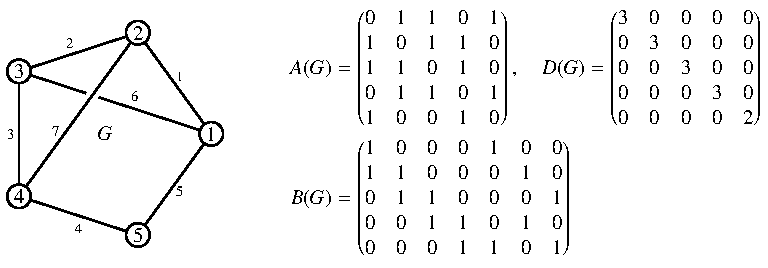
\includegraphics{chapters/70-graphen/images/adjazenzu.pdf}
\caption{Adjazenz-, Inzidenz- und Gradmatrix eines ungerichteten
Graphen mit $5$ Knoten und $7$ Kanten.
\label{buch:graphen:fig:adjazenzu}}
\end{figure}
Eine naheliegende Beschreibung eines Graphen mit Hilfe einer
Matrix kann man wie folgt erhalten.
Zunächst werden die Knoten aus der Menge $V$ durch die Zahlen
$1,\dots,n$ mit $n=|V|$ ersetzt.
Diese Zahlen werden dann als Zeilen- uns Spaltenindizes interpretiert.
Die zum Graphen gehörige sogenannte {\em Adjazenzmatrix} $A(G)$
enthält die Einträge
\begin{equation}
a_{ij}
=
\begin{cases}
1&\qquad  \{j,i\} \in E\\
0&\qquad  \text{sonst.}
\end{cases}
\label{buch:graphen:eqn:linkmatrix}
\end{equation}
Die Matrix hat also genau dann einen von Null verschiedenen Eintrag
in Zeile $i$ und Spalte $j$, wenn die beiden Knoten $i$ und $j$
im Graphen verbunden sind.
Die Adjazenzmatrix eines ungerichteten Graphen ist immer symmetrisch.
Ein Beispiel ist in Abbildung~\ref{buch:graphen:fig:adjazenzu}
dargestellt.

\begin{figure}
\centering
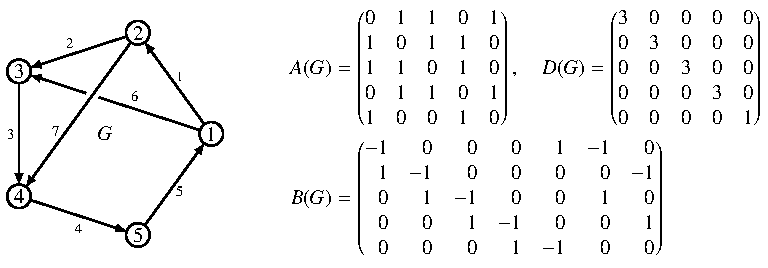
\includegraphics{chapters/70-graphen/images/adjazenzd.pdf}
\caption{Adjazenz-, Inzidenz- und Gradmatrix eines gerichteten
Graphen mit $5$ Knoten und $7$ Kanten.
\label{buch:graphen:fig:adjazenzd}}
\end{figure}
Die Adjazenzmatrix kann auch für einen gerichteten Graphen definiert
werden wie dies in in Abbildung~\ref{buch:graphen:fig:adjazenzu}
illustriert ist.
Ihre Einträge sind in diesem Fall definiert mit Hilfe der 
gerichteten Kanten als
\begin{equation}
A(G)_{ij}
=
a_{ij}
=
\begin{cases}
1&\qquad  (j,i) \in E\\
0&\qquad  \text{sonst.}
\end{cases}
\label{buch:graphen:eqn:linkmatrix}
\end{equation}
Die Matrix $A(G)$ hat also genau dann einen nicht verschwindenden
Matrixeintrag in Zeile $i$ und Spalte $j$, wenn es eine Verbindung
von Knoten $j$ zu Knoten $i$ gibt.

% XXX Abbildung Graph und Verbindungs-Matrix

\subsubsection{Adjazenzmatrix und die Anzahl der Pfade}
Die Beschreibung des Graphen mit der Adjazenzmatrix $A=A(G)$ nach
\eqref{buch:graphen:eqn:linkmatrix} ermöglicht bereits, eine interessante
Aufgabe zu lösen.

\begin{satz}
\label{buch:graphen:pfade-der-laenge-n}
Der gerichtete Graph $G=([n],E)$ werde beschrieben durch die Adjazenzmatrix
$A=A(G)$.
Dann gibt das Element in Zeile $j$ und Spalte $i$ von $A^n$ die Anzahl
der Wege der Länge $n$ an, die von Knoten $i$ zu Knoten $j$ führen.
Insbesondere kann man die Definition~\eqref{buch:graphen:eqn:linkmatrix}
formulieren als: In Zeile $j$ und Spalte $i$ der Matrix steht die Anzahl
der Pfade der Länge $1$, die $i$ mit $j$ verbinden.
\end{satz}

\begin{proof}[Beweis]
Es ist klar, dass $A^1$ die genannte Eigenschaft hat.
Wir beweisen, dass $A^n$ Pfade der Länge $n$ zählt, mit Hilfe von
vollständiger Induktion.
Zur Unterscheidung schreiben wir $A^{(n)}$ für die Matrix, die in Zeile
$j$ und Spalte $i$ die Anzahl der Pfade der Länge $n$ von $i$ nach $j$
enhält.
Die zugehörigen Matrixelemente schreiben wir $a_{ji}^{n}$ bzw.~$a_{ji}^{(n)}$.
Wir haben also zu zeigen, dass $A^n = A^{(n)}$.

Wir nehmen daher an, dass bereits bewiesen ist, dass das Element in Zeile
$j$ und Spalte $i$ von $A^{n-1}$ die Anzahl der Pfade der Länge $n-1$
zählt, dass also $A^{n-1}=A^{(n-1)}$.
Dies ist die Induktionsannahme.

Wir bilden jetzt alle Pfade der Länge $n$ von $i$ nach $k$.
Ein Pfad der Länge besteht aus einem Pfad der Länge $n-1$, der von $i$ zu
einem beliebigen Knoten $j$ führt, gefolgt von einer einzelnen Kante,
die von $j$ nach $k$ führt.
Ob es eine solche Kante gibt, zeigt das Matrixelement $a_{kj}$ an.
Das Element in Zeile $j$ und Spalte $i$ der Matrix $A^{(n-1)}$ gibt
die Anzahl der Wege von $i$ nach $j$ an.
Es gibt also $a_{kj}\cdot a_{ji}^{(n-1)}$ Wege der Länge $n$, die von $i$
nach $k$ führen, aber als zweitletzten Knoten über den Knoten $j$ führen.
Die Gesamtzahl der Wege der Länge $n$ von $i$ nach $k$ ist daher
\[
a_{ki}^{(n)}
=
\sum_{j=1}^n a_{kj} a_{ji}^{(n-1)}.
\]
In Matrixschreibweise bedeutet dies
\[
A^{(n)}
=
A\cdot A^{(n-1)}
=
A\cdot A^{n-1}
=
A^n.
\]
Beim zweiten Gleichheitszeichen haben wir die Induktionsannahme
verwendet.
\end{proof}

Der Satz~\ref{buch:graphen:pfade-der-laenge-n} ermöglicht auch, einen 
Algorithmus für den sogenannten Durchmesser eines Graphen zu formulieren.

\begin{definition}
\index{Durchmesser eines Graphen}%
\index{Graph!Durchmesser des}%
Der {\em Durchmesser} eines Graphen ist die kürzeste Länge $d$ derart, dass
es zwischen zwei beliebigen Knoten einen Pfad der Länge $\le d$ gibt.
\end{definition}

Der Durchmesser $d$ eines Graphen ist der kleinste Exponent derart,
dass $A^d$ keine ausserdiagonalen Einträge $0$ hat.
Die Diagonalelemente von $A^n$ zählen die Anzahl der geschlossenen Pfade
der Länge $n$, die durch einen Knoten führen.
Diese können für den Durchmesser ignoriert werden.
Man kann also Potenzen $A^n$ berechnen bis keine Einträge $0$ mehr vorhanden
sind.

\begin{beispiel}
\begin{figure}
\centering
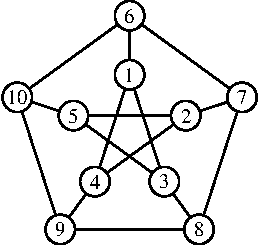
\includegraphics{chapters/70-graphen/images/peterson.pdf}
\caption{Peterson-Graph mit zehn Knoten.
\label{buch:figure:peterson}}
\end{figure}
Der Peterson-Graph hat die Adjazenzmatrix
\[
G
=
\begin{pmatrix}
%1  2  3  4  5  6  7  8  9 10
 0& 0& 1& 1& 0& 1& 0& 0& 0& 0\\ %  1
 0& 0& 0& 1& 1& 0& 1& 0& 0& 0\\ %  2
 1& 0& 0& 0& 1& 0& 0& 1& 0& 0\\ %  3
 1& 1& 0& 0& 0& 0& 0& 0& 1& 0\\ %  4
 0& 1& 1& 0& 0& 0& 0& 0& 0& 1\\ %  5
 1& 0& 0& 0& 0& 0& 1& 0& 0& 1\\ %  6
 0& 1& 0& 0& 0& 1& 0& 1& 0& 0\\ %  7
 0& 0& 1& 0& 0& 0& 1& 0& 1& 0\\ %  8
 0& 0& 0& 1& 0& 0& 0& 1& 0& 1\\ %  9
 0& 0& 0& 0& 1& 1& 0& 0& 1& 0   % 10
\end{pmatrix}
\]
Durch Nachrechnen kann man bestätigen, dass $G^3$ keine
Ausserdiagonalelemente $0$ enthält:
\[
G^3
=
\begin{pmatrix}
 0& 2& 5& 5& 2& 5& 2& 2& 2& 2\\
 2& 0& 2& 5& 5& 2& 5& 2& 2& 2\\
 5& 2& 0& 2& 5& 2& 2& 5& 2& 2\\
 5& 5& 2& 0& 2& 2& 2& 2& 5& 2\\
 2& 5& 5& 2& 0& 2& 2& 2& 2& 5\\
 5& 2& 2& 2& 2& 0& 5& 2& 2& 5\\
 2& 5& 2& 2& 2& 5& 0& 5& 2& 2\\
 2& 2& 5& 2& 2& 2& 5& 0& 5& 2\\
 2& 2& 2& 5& 2& 2& 2& 5& 0& 5\\
 2& 2& 2& 2& 5& 5& 2& 2& 5& 0
\end{pmatrix}
\]
Daraus kann man jetzt ablesen, dass der Durchmesser des Petersongraphen
$d=5$ ist.
Man kann aber auch mehr ablesen:
\begin{itemize}
\item
Es gibt keine geschlossenen Pfade der Länge $\le 3$.
\item
Zwischen benachbarten Knoten gibt es jeweils $5$ Pfade der Länge $3$,
zwischen nicht benachbarten Knoten gibt es genau $2$ Pfade der Länge $3$.
\qedhere
\end{itemize}
\end{beispiel}

Das Beispiel illustriert, wie sich Zählaufgaben von Pfaden leicht mit dem
Matrizenprodukt erledigen lassen.
Trotzdem ist der Algorithmus nicht unbedingt effizient, da der Aufwand
zur Berechnung des Matrizenproduktes relativ gross sein kann.
Für den Peterson-Graphen können die gefundenen Aussagen über die Anzahl
von Pfaden durch Ausnützung der Symmetrien des Graphen leichter direkt
gefunden werden.

\subsubsection{Beschriftete Graphen}
Bei der Beschreibung eines elektrischen Netzwerkes mit Hilfe eines
ungerichteten Graphen muss jeder Kante zusätzlich ein Widerstandswert
zugeordnet werden.
Dies ist, was eine Beschriftung einer Kante bewerkstelligt.

\begin{definition}
Eine Beschriftung mit Elementen der Menge $L$
eines gerichteten oder ungerichteten Graphen $G=(V,E)$ 
ist eine Abbildung $l\colon E\to L$.
\index{Beschriftung}%
\end{definition}

\subsection{Inzidenzmatrix}
Die Adjazenzmatrix kann zusätzliche Information, die möglicherweise
mit den Kanten verbunden ist, nicht mehr darstellen.
Dies tritt zum Beispiel in der Informatik bei der Beschreibung
endlicher Automaten auf, wo zu jeder gerichteten Kante auch noch
Buchstaben gehören, für die der Übergang entlang dieser Kante
möglich ist.

Die {\em Inzidenzmatrix} löst dieses Problem.
\index{Inzidenzmatrix}%
Dazu werden zunächst die Kanten numeriert $1,\dots,m$
numeriert.
Die Matrixeinträge
\[
a_{ij} = \begin{cases}
1\qquad&\text{Knoten $i$ ist ein Endpunkt von Kante $j$}
\\
0\qquad&\text{sonst}
\end{cases}
\]
stellen die Beziehung zwischen Kanten und Knoten her.

\subsubsection{Beschriftete Graphen}
Die Inzidenzmatrix kann auch einen erweiterten Graphenbegriff abbilden,
in dem zwischen zwei Kanten mehrere Verbindungen möglich sind.
Graphen mit beschrifteten Kanten gehören dazu.

\begin{definition}
Ein gerichteter Graph mit beschrifteten Kanten ist eine Menge $V$ von 
Knoten und eine Menge von beschrifteten Kanten der Form
\[
E \{ (a,b,l)\in V^2\times L\;|\; \text{Eine Kante mit Beschriftung $l$ führt von $a$ nach $b$}\}.
\]
Die Menge $L$ enthält die möglichen Beschriftungen der Kanten.
\end{definition}

Für einen gerichteten Graphen wird in der Inzidenzmatrix für
den Anfangspunkt einer Kante $-1$ eingetragen und für den
Endpunkt $+1$.
% XXX Beispiel

\subsubsection{Inzidenzmatrix und Adjazenzmatrix}
Sei $B(G)$ die Inzidenzmatrix eines Graphen $G$. 
Die Spalten von $B(G)$ sind mit den Kanten des Graphen indiziert.
Die Matrix $B(G)B(G)^t$ ist eine quadratische Matrix, deren
Zeilen und Spalten mit den Knoten des Graphen indiziert sind.
In dieser Matrix geht die Informatione über die individuellen
Kanten wieder verloren.
Sie hat für $i\ne j$ die Einträge
\begin{align*}
(B(G)B(G)^t)_{ij}
&=
\sum_{\text{$k$ Kante}} b_{ik}b_{jk}
\\
&=\text{Anzahl der Kanten, die $i$ mit $j$ verbinden}
\\
&=a_{ij}
\end{align*}
Die Adjazenzmatrix eines Graphen lässt sich also aus der
Inzidenzmatrix berechnen.

\subsubsection{Gradmatrix}
\index{Gradmatrix}%
Die Diagonale von $B(G)B(G)^t$ enthält die Werte
\begin{align*}
(B(G)B(G)^t)_{ii}
&=
\sum_{\text{$k$ Kante}} b_{ik}^2
=
\text{Anzahl Kanten, die im Knoten $i$ enden}
\end{align*}
Der {\em Grad} eines Knoten eines Graphen ist die Anzahl der
\index{Grad eines Knotens}%
Kanten, die in diesem Knoten enden.
Die Diagonalmatrix die aus den Graden der Knoten besteht, heisst die
Gradmatrix $D(G)$ des Graphen.
Es gilt daher $B(G)B(G)^t = A(G) + D(G)$.

\subsubsection{Gerichtete Graphen}
Für einen gerichteten Graphen ändert sich an der Diagonalen
der Matrix $B(G)B(G)^t$ nichts.
Da es in einem gerichteten Graphen nur eine einzige Kante $k$ gibt, die zwei
Knoten $i$ und $j$ verbinden kann, muss das zugehörige 
Ausserdiagonalelement
\[
a_{ij}
=b_{ik}b_{jk}
=
-1
\]
sein.
Für einen gerichteten Graphen sind daher alle Ausserdiagonalelemente
negativ und es gilt $B(G)B(G)^t = D(G)-A(G)$.

\subsubsection{Anwendung: Netlist}
Eine natürliche Anwendung eines gerichteten und beschrifteten Graphen
ist eine eletronische Schaltung.
Die Knoten des Graphen sind untereinander verbundene Leiter, sie werden
auch {\em nets} genannt. 
Die beschrifteten Kanten sind die elektronischen Bauteile, die solche
Nets miteinander verbinden.
Die Inzidenzmatrix beschreibt, welche Anschlüsse eines Bauteils mit
welchen Nets verbunden werden müssen.
Die Informationen in der Inzidenzmatrix werden also in einer
Applikation zum Schaltungsentwurf in ganz natürlicher Weise erhoben.

\subsection{Die Adjazenzmatrix und Laplace-Matrix
\label{subsection:adjazenz-und-laplace-matrix}}
Die Beschreibung mit der Matrix~\eqref{buch:graphen:eqn:linkmatrix}
``vergisst'' den ``Namen'' der Kante, die eine Verbindung zwischen zwei
Knoten herstellt.
Damit ist sie keine geeignete Grundlage, um beschriftete Graphen einer
Matrixbeschreibung zuzuführen.
Eine solche muss eine Matrix verwenden, die nicht nur das Vorhandensein einer
Verbindung wiedergibt, sondern ausdrückt, welche Kante welche beiden
Knoten miteinander verbindet.
Dies führt zur sogenannten Adjazenzmatrix.

\begin{definition}
\label{buch:def:adjazenz-matrix}
Ist $G=(V,E)$ ein gerichteter Graph mit $n=|G|$ Vertizes und $m=|E|$ Kanten,
dann ist die zugehörige {\em Adjazenzmatrix} $A=A(G)$ eine $n\times m$-Matrix.
In der Spalte $k$ wird der Anfangspunkt der Kante $k$ mit $-1$, der Endpunkt
mit $+1$ angezeigt, die übrigen Einträge sind $0$.
$A$ hat also die Matrixelemente
\begin{equation}
a_{ik}
=
\begin{cases}
-1&\qquad i=a(k)\\
+1&\qquad i=e(k)\\
\phantom{+}0&\qquad\text{sonst}
\end{cases}
\label{buch:eqn:ajazenz-matrix}
\end{equation}
\end{definition}

Der wesentliche Unterschied dieser Definition von der Matrix $G$
liegt in der Bedeutung der Einträge.
Für $G$ drückt ein nicht verschwindendes Matrixelement das Vorhandensein
einer Kante aus, in $A$ ist es die Tatsache, dass in diesem Knoten
eine Kante beginnt oder endet.

Es ist natürlich möglich, aus der Adjazenzmatrix auch die Link-Matrix
zu rekonstruieren.
Dazu muss für jedes Paar $(j,i)$ von Knoten festgestellt werden,
ob die Adjazenzmatrix eine entsprechende Verbindung enthält, also ob der
Vektor 
\[
k_{ji} = e_i - e_j
\]
als Spaltenvektor vorkommt, wobei die $e_i$ die $n$-dimensionalen
Standardbasisvektoren sind.



%
% spektral.tex
%
% (c) 2020 Prof Dr Andreas Müller, Hochschule Rapperswil
%
\section{Spektrale Graphentheorie
\label{buch:section:spektrale-graphentheorie}}
\rhead{Spektrale Graphentheorie}

%
% wavelets.tex -- Wavelets auf Graphen
%
% (c) 2020 Prof Dr Andreas Müller, Hochschule Rapperswil
%
\section{Wavelets auf Graphen
\label{buch:section:wavelets-auf-graphen}}
\rhead{Wavelets auf Graphen}
In Abschnitt~\ref{buch:subsection:standardbasis-und-eigenbasis} wurde
gezeigt dass die Standardbasis den Zusammenhang zwischen den einzelnen
Teilen des Graphen völlig ignoriert, während die Eigenbasis Wellen
beschreibt, die mit vergleichbarer Amplitude sich über den ganzen
Graphen entsprechen.
Die Eigenbasis unterdrückt also die ``Individualität'' der einzelnen
Knoten fast vollständig.

Wenn man einen Standardbasisvektor in einem Knoten $i$
als Anfangstemperaturverteilung verwendet, erwartet man eine Lösung,
die für kleine Zeiten $t$ die Energie immer in der Nähe des Knotens $i$
konzentriert hat.
Weder die Standardbasis noch die Eigenbasis haben diese Eigenschaft.

\subsection{Vergleich mit der Wärmeleitung auf $\mathbb{R}$}
Ein ähnliches Phänomen findet man bei der Wärmeausbreitung gemäss
der partiellen Differentialgleichung
\[
\frac{\partial T}{\partial t} = -\kappa \frac{\partial^2 T}{\partial x^2}.
\]
Die von Fourier erfundene Methode, die Fourier-Theorie, verwendet die
Funktionen $e^{ik x}$, die Eigenvektoren der zweiten Ableitung
$\partial^2/\partial x^2$ sind.
Diese haben das gleiche Problem, der Betrag von $e^{ikx}$ ist $1$, die
Entfernung von einem Punkt spielt überhaupt keine Rolle.
Die Funktion
\[
F(x,t)
=
\frac{1}{\sqrt{4\pi\kappa t}}e^{-x^2/4\kappa t}
\]
ist eine Lösung der Wärmeleitungsgleichung mit einem Maximum an
der Stelle $0$.
Sie heisst die Fundamentallösung der Wärmeleitungsgleichung.
Durch Überlagerung von Translaten in eine Funktion
\begin{equation}
f(x,t)
=
\int_{-\infty}^\infty f(\xi) F(x-\xi,t)\,d\xi
\label{buch:graphen:eqn:fundamentalueberlagerung}
\end{equation}
kann man die allgemeine Lösung aus Fundamentallösungen zusammensetzen.
Die Fundamentallösungen $f(x-\xi,t)$ sind für kleine Zeiten immer noch
deutlich in einer Umgebung von $\xi$ konzentriert.

% XXX Ausbreitung der Fundamentallösung illustrieren
\begin{figure}
\centering
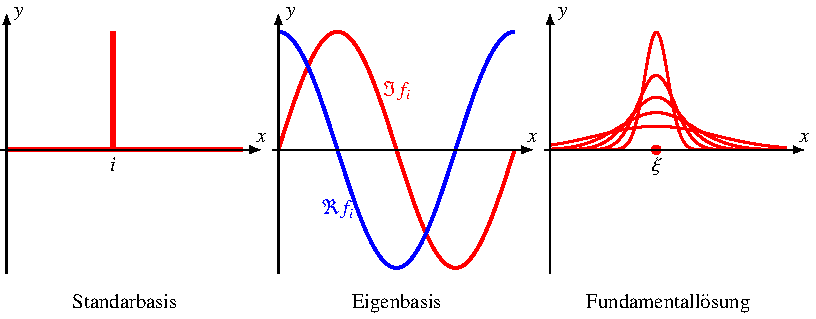
\includegraphics{chapters/70-graphen/images/fundamental.pdf}
\caption{Vergleich der verschiedenen Funktionenfamilien, mit denen
Lösungenfunktionen durch Linearkombination erzeugt werden können.
In der Standarbasis (links) ist es am einfachsten, die Funktionswerte
abzulesen, in der Eigenbasis (Mitte) kann die zeitliche Entwicklung
besonders leicht berechnet werden.
Dazuwischen liegen die Fundamentallösungen (rechts), die eine einigermassen
übersichtliche Zeitentwicklung haben, die Berechnung der Temperatur an 
einer Stelle $x$ zur Zeit $t$ ist aber erst durch das Integral
\eqref{buch:graphen:eqn:fundamentalueberlagerung} gegeben.
\label{buch:graphen:fig:fundamental}}
\end{figure}

\subsection{Fundamentallösungen auf einem Graphen}
Die Wärmeleitungsgleichung auf einem Graphen kann für einen
Standardbasisvektor mit Hilfe der
Lösungsformel~\eqref{buch:graphen:eqn:eigloesung}
gefunden werden.
Aus physikalischen Gründen ist aber offensichtlich, dass die
Wärmeenergie Fundamentallösungen $F_i(t)$ für kurze Zeiten $t$
in der Nähe des Knoten $i$ konzentriert ist.
Dies ist aber aus der expliziten Formel
\begin{equation}
F_i(t)
=
\sum_{j=1}^n \langle f_j,e_i\rangle e^{-\kappa \lambda_i t} f_j
=
\sum_{j=1}^n \overline{f}_{ji} e^{-\kappa \lambda_i t},
\label{buch:graphen:eqn:fundamentalgraph}
\end{equation}
nicht unmittelbar erkennbar.

Man kann aber aus~\eqref{buch:graphen:eqn:fundamentalgraph} ablesen,
dass für zunehmende Zeit die hohen Frequenzen sehr schnell gedämpft
werden.
Die hohen Frequenzen erzeugen also den scharfen Peak für Zeiten nahe
beim Knoten $i$, die zu kleineren $\lambda_i$ beschreiben die Ausbreitung
über grössere Distanzen.
Die Fundamentallösung interpoliert also in einem gewissen Sinne zwischen
den Extremen der Standardbasis und der Eigenbasis.
Die ``Interpolation'' geht von der Differentialgleichung aus,
sie ist nicht einfach nur ein Filter, der die verschiedenen Frequenzen
auf die gleiche Art bearbeitet.

Gesucht ist eine Methode, eine Familie von Vektoren zu finden,
aus der sich alle Vektoren linear kombinieren lassen, in der aber
auch auf die für die Anwendung interessante Längenskala angepasste
Funktionen gefunden werden können.

\subsection{Wavelets auf einem Graphen}
Die Fourier-Theorie analysiert Funktionen nach Frequenzen, wobei die 
zeitliche Position von interessanten Stellen der Funktion in der Phase
der einzelnen Komponenten verschwindet.
Die Lokalisierung geht also für viele praktische Zwecke verloren.
Umgekehrt haben einzelne Ereignisse wie eine $\delta$-Funktion keine
charakteristische Frequenz, sie sind daher im Frequenzraum überhaupt 
nicht lokalisierbar.
Die Darstellung im Frequenzraum und in der Zeit sind also extreme
Darstellungen, entweder Frequenzlokalisierung oder zeitliche Lokalisierung
ermöglichen, sich aber gegenseitig ausschliessen.

\subsubsection{Dilatation}
Eine Wavelet-Basis für die $L^2$-Funktionen auf $\mathbb{R}$ erlaubt
eine Funktion auf $\mathbb{R}$ auf eine Art zu analysieren, die eine
ungenaue zeitliche Lokalisierung bei entsprechend ungenauer
Frequenzbestimmung ermöglicht.
Ausserdem entstehen die Wavelet-Funktionen aus einer einzigen Funktion
$\psi(t)$ durch Translation um $b$ und Dilatation mit dem Faktor $a$:
\[
\psi_{a,b}(t)
=
\frac{1}{\sqrt{|a|}} \psi\biggl(\frac{t-b}a\biggr)
=
T_bD_a\psi(t)
\]
in der Notation von \cite{buch:mathsem-wavelets}.
Auf einem Graphen ist so eine Konstruktion grundsätzlich nicht möglich,
da es darauf weder eine Translations- noch eine Streckungsoperation gibt.

In der Theorie der diskreten Wavelet-Transformation ist es üblich, sich
auf Zweierpotenzen als Streckungsfaktoren zu beschränken.
Ein Gitter wird dadurch auf sich selbst abgebildet, aber auf einem
Graphen gibt es keine Rechtfertigung für diese spezielle Wahl von
Streckungsfaktoren mehr.
Es stellt sich daher die Frage, ob man für eine beliebige Menge
\(
T= \{ t_1,t_2,\dots\} \}
\)
von Streckungsfaktoren eine Familie von Funktionen $\chi_j$ zu finden
derart, dass man sich die $\chi_j$ in einem gewissen Sinn als aus
$\chi_0$ durch Dilatation entstanden vorstellen kann.

Die Dilatation kann natürlich nicht von einer echten
Dilatation im Ortsraum herstammen, aber man kann wenigstens versuchen, die
Dilatation im Frequenzraum nachzubilden.
Für Funktionen in $L^2(\mathbb{R})$ entspricht die Dilatation mit dem
Faktor $a$ im Ortsraum der Dilatation mit dem Faktor $1/a$ im Frequenzraum:
\[
\widehat{D_af}(\omega) = D_{1/a}\hat{f}(\omega).
\]
\cite[Satz~3.14]{buch:mathsem-wavelets}.
Es bleibt aber das Problem, dass sich auch die Skalierung im Frequenzraum
nicht durchführen lässt, da auch das Frequenzspektrum des Graphen nur eine
Menge von reellen Zahlen ohne innere algebraische Struktur ist.

\subsubsection{Mutterwavelets}
\begin{figure}
\centering
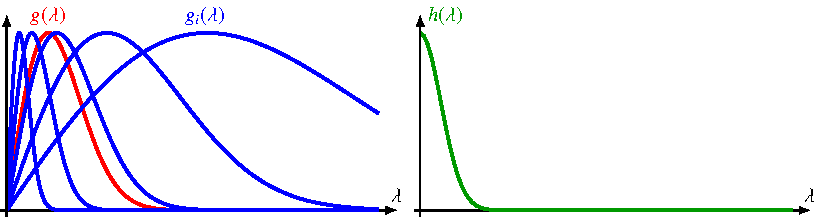
\includegraphics{chapters/70-graphen/images/gh.pdf}
\caption{Lokalisierungsfunktion $g(\lambda)$ für die Dilatation (links).
Die Dilatierten Funktionen $g_i=\tilde{D}_{1/a_i}g$ lokalisieren
die Frequenzen jeweils um die Frequenzen $a_i$ im Frequenzraum.
Der Konstante Vektor ist vollständig delokalisiert, die Funktion $h$
in der rechten Abbildung entfernt die hohen Frequenzen und liefert Funktionen,
die in der Umgebung eines Knotens wie die Konstante Funktion aussehen.
\label{buch:graphs:fig:lokalisierung}}
\end{figure}
Das Mutter-Wavelet einer Wavelet-Analyse zeichnet definiert, in welchem Mass
sich Funktionen im Orts- und im Frequenzraum lokalisieren lassen.
Die Standardbasis der Funktionen auf einem Graphen repräsentieren die
perfekte örtliche Lokalisierung, Eigenbasis der Laplace-Matrix repräsentiert
die perfekte Lokalisierung im Frequenzraum.
Sei $g(\lambda)\ge 0$ eine Funktion im Frequenzraum, die für  $\lambda\to0$ und
$\lambda\to\infty$ rasch abfällt mit einem Maximum irgendwo dazwischen
(Abbildung~\ref{buch:graphs:fig:lokalisierung}).
Sie kann als eine Lokalisierungsfunktion im Frequenzraum betrachtet werden.

Die Matrix $g(I)$ bildet entfernt aus einer Funktion die ganz hohen und 
die ganz tiefen Frequenz, lokalisiert also die Funktionen im Frequenzraum.
Die Standardbasisvektoren werden dabei zu Funktionen, die nicht mehr nur
auf einem Knoten von $0$ verschieden sind, aber immer noch einigermassen
auf dem Graphen lokalisiert sind.
Natürlich sind vor allem die Werte auf den Eigenwerten
$\lambda_0 < \lambda_1\le \dots\le \lambda_n$ der Laplace-Matrix
von Interesse.

Die Matrix $g(I)$ kann mit Hilfe der Spektraltheorie berechnet werden,
was im vorliegenden Fall naheliegend ist, weil ja die Eigenvektoren von
der Laplace-Matrix bereits bekannt sind.
Die Matrix $\chi^t$ bildet die Standardbasisvektoren in die
Eigenbasis-Vektoren ab, also in eine Zerlegung im Frequenzraum ab,
$\chi$ vermittelt die Umkehrabbildung.
Mit der Spektraltheorie findet man für die Abbildung $g(I)$ die Matrix
\begin{equation}
g(I)
=
\chi
\begin{pmatrix}
g(\lambda_0)&0&\dots&0\\
0&g(\lambda_1)&\dots&0\\
\vdots&\vdots&\ddots&\vdots\\
0&0&\dots&g(\lambda_n)
\end{pmatrix}
\chi^t.
\label{buch:graphen:eqn:mutterwavelet}
\end{equation}

\subsubsection{Dilatation}
Die Dilatation um $a$ im Ortsraum wird zu einer Dilatation um $1/a$ im
Frequenzraum.
Statt also nach einer echten Dilatation der Spaltenvektoren in $g(I)$
zu suchen, kann man sich darauf verlegen, Funktionen zu finden, deren
Spektrum von einer Funktionen lokalisiert worden ist, die eine Dilatation
von $g$ ist.
Man wählt daher eine ansteigende Folge $A=(a_1,\dots)$ von Streckungsfaktoren
und betrachtet anstelle von $g$ die dilatierten Funktionen
$g_i=\tilde{D}_{1/a_i}g$.
Die zugehörigen Wavelet-Funktionen auf dem Graphen können wieder mit
der Formel~\eqref{buch:graphen:eqn:mutterwavelet} berechnet werden,
man erhält
\begin{equation}
\tilde{D}_{1/a_i}g(I)
=
g_i(I)
=
\chi
\begin{pmatrix}
g(a_i\lambda_0)&0&\dots&0\\
0&g(a_i\lambda_1)&\dots&0\\
\vdots&\vdots&\ddots&\vdots\\
0&0&\dots&g(a_i\lambda_n)
\end{pmatrix}
\chi^t .
\end{equation}
Die Spalten von $g_i(I)$ bilden wieder eine Menge von Funktionen, die
eine gemäss $g_i$ lokalisiertes Spektrum haben.

\subsubsection{Vater-Wavelet}
Wegen $g(0)=0$ wird die konstante Funktion, die Eigenvektor zum Eigenwert
$\lambda_0=0$ ist, von den Abbildungen $g_i(I)$ auf $0$ abgebildet.
Andererseits ist diese Funktion nicht lokalisiert, man möchte Sie also
für die Analyse nicht unbedingt verwenden.
Man wählt daher eine Funktion $h(\lambda)$ mit $h(0)=1$ so, dass
für $\lambda\to \infty$ der Wert $h(\lambda)$ genügend rasch gegen $0$
geht.
Die Matrix $h(I)$ bildet daher den konstanten Vektor nicht auf $0$ ab,
sondern lokalisiert ihn im Ortsraum.
Wir erhalten daher in den Spalten von $h(I)$ Vektoren, die um die
einzelnen Knoten lokalisiert sind.

\subsubsection{Rekonstruktion}
Die Operatoren $h(I)$ und $g_i(I)$ erzeugen analysieren eine Funktion
nach den verschiedenen Frequenzen mit den Skalierungsfaktoren $a_i$,
aber die Rekonstruktion ist noch nicht klar.
Diese wäre einfacher, wenn die Operatoren zusammen die identische
Abbildung ergäben, wenn also
\[
h(I) + \sum_{i}g_i(I)=I
\]
gelten würde.
Nach der Spektraltheorie gilt das nur, wenn für alle Eigenwerte
$\lambda_k$, $k=1,\dots,n$
\[
h(\lambda_k) + \sum_ig(a_i\lambda_k)=1
\]
gilt.
Für beleibige Funktionen $g$ und $h$ kann man nicht davon ausgehen,
aber man kann erwarten.
Man muss daher zusätzlich verlangen, dass
\[
h(\lambda_k) + \sum_{i} g(a_i\lambda_k) > 0
\]
ist für alle Eigenwerte $\lambda_k$.

\subsubsection{Frame}
Die Menge von Vektoren, die in der vorangegangenen Konstruktion gefunden
wurden, ist zu gross, um eine Basis zu sein.
Vektoren lassen sich darin auf verschiedene Art darstellen.
Wir verlangen aber auch keine eindeutige Darstellung, nur eine 
Darstellung, in der wir die ``dominierenden'' Komponenten in jeder
Frequenzskala identifizieren können.

\begin{definition}
\label{buch:graphen:def:frame}
Ein Frame des Vektorraumes $\mathbb{R}^n$ ist eine Menge
$F=\{e_k\;|\; k=1,\dots,N\}$ von Vektoren mit der Eigenschaft
\begin{equation}
A\|v\|^2
\le
\sum_{k=1}^N  |\langle v,e_k\rangle|^2
\le
B\|v\|^2
\label{buch:graphen:eqn:frame}
\end{equation}
Die Zahlen $A$  und $B$ heissen die {\em Frame-Konstanten} des Frames.
\end{definition}

Die oben gefundenen Vektoren, die Spalten Vektoren von $h(I)$ und $g_i(I)$
bilden daher ein Frame.
Die Frame-Konstanten kann man unmittelbar ausrechnen.
Der mittlere Term von \eqref{buch:graphen:eqn:frame} ist 
\[
\|h(I) v\|^2
+
\sum_{i} \|g_i(I)v\|^2,
\]
die durch die Funktion
\[
f(\lambda)
=
h(\lambda)^2 + \sum_i g_i(\lambda)^2
\]
abgeschätzt werden kann.
Die Frame-Konstanten sind daher
\begin{align*}
A&=\min_{k} f(\lambda_k)
&
&\text{und}&
B&=\max_{k} f(\lambda_k).
\end{align*}
Die Konstruktion hat also ein Frame für die Funktionen auf dem Graphen
etabliert, die viele Eigenschaften einer Multiskalenanalyse in diese
wesentlich weniger symmetrische Situation rettet.






